\subsection*{Numpy Introduction}

\begin{frame}[fragile]
How slow is Python?  Let's add one to a million numbers.

\begin{block}{Using lists}
\begin{minted}{python}
In [15]: lst = range(1000000)

In [16]: %timeit [i + 1 for i in lst]
10 loops, best of 3: 65.6 ms per loop
\end{minted}
\end{block}

\begin{block}{Using NumPy}
\begin{minted}{python}
In [18]: arr = arange(1000000)

In [19]: %timeit arr + 1
100 loops, best of 3: 2.91 ms per loop
\end{minted}
\end{block}
\end{frame}

\begin{frame}
  What makes an array so much faster?
  \begin{itemize}
  \item Data layout
    \begin{itemize}
    \item homogenous: every item takes up the same size block of memory
    \item single data-type objects
    \item powerful array scalar types
    \end{itemize}
  \item universal function (ufuncs)
    \begin{itemize}
    \item function that operates on ndarrays in an element-by-element fashion
    \item vectorized wrapper for a function
    \item built-in functions are implemented in compiled C code
    \end{itemize}
\end{itemize}
\end{frame}

\begin{frame}
  Data layout
  \begin{itemize}
  \item homogenous: every item takes up the same size block of memory
  \item single data-type objects
  \item powerful array scalar types
  \end{itemize}
  \begin{center}
    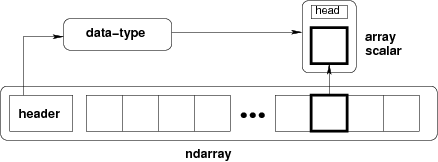
\includegraphics[scale=.5]{../figures/numpy/threefundamental.png}
  \end{center}
\end{frame}

\begin{frame}[fragile]
  universal function (ufuncs)
  \begin{itemize}
  \item function that operates on ndarrays in an element-by-element fashion
  \item vectorized wrapper for a function
  \item built-in functions are implemented in compiled C code
  \end{itemize}
  \begin{block}{python function v ufunc}
    \begin{minted}{python}
In [31]: %timeit [sin(i)**2 for i in arr]
1 loops, best of 3: 4.32 s per loop

In [32]: import numpy as np

In [33]: %timeit np.sin(arr)**2
10 loops, best of 3: 20.8 ms per loop
    \end{minted}
  \end{block}
\end{frame}

